\documentclass{article}

% set font encoding for PDFLaTeX, XeLaTeX, or LuaTeX
\usepackage{ifxetex,ifluatex}
\if\ifxetex T\else\ifluatex T\else F\fi\fi T%
  \usepackage{fontspec}
\else
  \usepackage[T1]{fontenc}
  \usepackage[utf8]{inputenc}
  \usepackage{lmodern}
\fi

\usepackage{hyperref}

\title{A Comparison of Image Segmentation Methods}
\author{Marshall Grimmett}

% Enable SageTeX to run SageMath code right inside this LaTeX file.
% http://doc.sagemath.org/html/en/tutorial/sagetex.html
% \usepackage{sagetex}

% Enable PythonTeX to run Python – https://ctan.org/pkg/pythontex
% \usepackage{pythontex}

\usepackage{amsmath}
\usepackage{pgfplots}
\pgfplotsset{compat=1.8}
\usepgfplotslibrary{statistics}

\usepackage{pgfplotstable}
\makeatletter
\long\def\ifnodedefined#1#2#3{%
    \@ifundefined{pgf@sh@ns@#1}{#3}{#2}%
}

\pgfplotsset{
    discontinuous/.style={
    scatter,
    scatter/@pre marker code/.code={
        \ifnodedefined{marker}{
            \pgfpointdiff{\pgfpointanchor{marker}{center}}%
             {\pgfpoint{0}{0}}%
             \ifdim\pgf@y>0pt
                \tikzset{options/.style={mark=*, fill=white}}
                \draw [densely dashed,blue] (marker-|0,0) -- (0,0);
                \draw plot [mark=*] coordinates {(marker-|0,0)};
             \else
                \tikzset{options/.style={mark=none}}
             \fi
        }{
            \tikzset{options/.style={mark=none}}
        }
        \coordinate (marker) at (0,0);
        \begin{scope}[options]
    },
    scatter/@post marker code/.code={\end{scope}}
    }
}

\makeatother

\begin{document}
\setlength{\parindent}{0pt}
\maketitle

% \begin{figure}[h!]
%   \includegraphics[width=\linewidth]{psi_0.1_epsilon_0.5.png}
% \end{figure}

% \newpage

% \begin{equation*}
%   z_j=c\times(w_j^{h^T}\bar{x})=c\times(\sum_{i=1}^{n}w_{ij}^hx_i+
%   b_{j}^hx_0)
% \end{equation*}

% \begin{multline*}
%   o_1=c\times(w_{11}^oz_1+w_{21}^oz_2) \\
%   =c\times(w_{11}^o(c\times(w_{11}^hx_1+w_{21}^hx_2+2b_1^hx_0))+
%   w_{21}^o(c\times(w_{12}^hx_1+w_{22}^hx_2+2b_2^hx_0))) \\
%   =c^2\times((w_{11}^ow_{11}^hx_1+w_{11}^ow_{21}^hx_2+2w_{11}^ob_1^hx_0)+
%   (w_{21}^ow_{12}^hx_1+w_{21}^ow_{22}^hx_2+2w_{21}^ob_2^hx_0)) \\
%   =c^2\times((w_{11}^ow_{11}^h+w_{21}^ow_{12}^h)x_1+
%   (w_{11}^ow_{21}^h+w_{21}^ow_{22}^h)x_2+(2w_{11}^ob_1^h+2w_{21}^ob_2^h)x_0)
% \end{multline*}

%%%%%%%%%%%%%%%%%%%%%%%%%%%%%%%%%%%%%%%%%%%%%%%%%%%%%%%%%%%%%%%%%%%%%%%%%%%%%%
\section{Part 1}

\subsection{a}
The new objective function, where $\alpha_i$ is a lagrangian multiplier
for each constraint, will be
\begin{equation*}
  min\ L = \frac{1}{2}w^2 - \sum_{i=1}^{n}\alpha_i(y_i(w^T \phi(x_i)) - 1)
\end{equation*}

\subsection{b}
Taking the derivative of $L$ with respect to $w$ we get
\begin{equation*}
  \frac{\partial}{\partial w} L = w - \sum_{i=1}^{n}\alpha_i y_i \phi(x_i)
\end{equation*}

\subsection{c}
Setting the derivative to zero and solving for $w$ gives us
\begin{equation*}
  \frac{\partial}{\partial w} L = w - \sum_{i=1}^{n}\alpha_i y_i \phi(x_i) = 0 \\
\end{equation*}
\begin{equation*}
w = \sum_{i=1}^{n}\alpha_i y_i \phi(x_i)
\end{equation*}
This allows us to replace $w$ in our objective function as a linear combination
of the data points in feature space, $\phi(x_i)$, and the signed Lagrange
multipliers, $\alpha_i y_i$ as coefficients. 

\subsection{d}
Substituting $w$ into our objective function will give us
\begin{multline*}
  L = \frac{1}{2}(\sum_{i=1}^{n}\alpha_i y_i \phi(x_i))^2 -
    \sum_{i=1}^{n}\alpha_i(y_i(\sum_{j=1}^{n}\alpha_j y_j \phi(x_j) )\phi(x_i)) - 1) \\
  = \frac{1}{2}\sum_{i=1}^{n}\alpha_i y_i \phi(x_i) \sum_{j=1}^{n}\alpha_j y_j \phi(x_j) -
    \sum_{i=1}^{n}\sum_{j=1}^{n}\alpha_i \alpha_j y_i y_j \phi(x_i)^T \phi(x_j) - \alpha_i \\
  = \frac{1}{2}\sum_{i=1}^{n}\sum_{j=1}^{n}\alpha_i \alpha_j y_i y_j \phi(x_i)^T \phi(x_j) -
    \sum_{i=1}^{n}\sum_{j=1}^{n}\alpha_i \alpha_j y_i y_j \phi(x_j)^T \phi(x_i) + \sum_{i=1}^{n}\alpha_i \\
  = \sum_{i=1}^{n}\alpha_i - \frac{1}{2}\sum_{i=1}^{n}\sum_{j=1}^{n}\alpha_i \alpha_j y_i y_j \phi(x_i)^T \phi(x_j)
\end{multline*}
So the new objective function will be
\begin{equation*}
  max_{\alpha}\ L_{dual} = \sum_{i=1}^{n}\alpha_i -
    \frac{1}{2}\sum_{i=1}^{n}\sum_{j=1}^{n}\alpha_i \alpha_j y_i y_j K(x_i, x_j)
\end{equation*}
subject to $\alpha_i \geq 0\ \forall i \in D$

\subsection{e}
let $J(\alpha)=L_{dual}$ then taking the partial derivative with repect to one
of the Lagrange multipliers we get
\begin{equation*}
  \frac{\partial J(\alpha_k)}{\partial \alpha_k} = 1 -
    y_k\sum_{i=1}^{n} \alpha_i y_i K(x_i, x_k)
\end{equation*}

\subsection{f}
After calculating all of the Lagrange multipliers we can compute $w$ using the
formula we derived from part (c)
\begin{equation*}
  w = \sum_{i=1}^{n}\alpha_i y_i \phi(x_i)
\end{equation*}
We can then calculate the class of a new point $z$ as
\begin{equation*}
  y = sign(w^T \phi(z)) = sign(\sum_{\alpha_i \ge 0}\alpha_i y_i K(x_i, z))
\end{equation*}

\subsection{g}
Picture (a) can not represent hard-margin kernel SVM since the
dataset is non-seperable. I.e. there is a red data point inside the circle
with the blue data points. \\
Picture (b) can represent hard-margin kernel SVM since the dataset is seperable
and the kernel will just be a linear kernel. \\
Picture (c) can represent hard-margin kernel SVM since the dataset is seperable
and the kernel will just be a quadratic kernel.\\
Picture (d) can not represent hard-margin kernel SVM since the dataset is
non-seperable. I.e. There are 2 data points which lie on the seperating
hyperplane so they cannot be classified.

%%%%%%%%%%%%%%%%%%%%%%%%%%%%%%%%%%%%%%%%%%%%%%%%%%%%%%%%%%%%%%%%%%%%%%%%%%%%%%
\section{Part 2}

\subsection{a}
(1)
\begin{equation*}
  W(S_1, T_1) = 4
\end{equation*}
\begin{equation*}
  W(S_2, T_2) = 2 + 3 = 5
\end{equation*}
\begin{equation*}
  W(S_3, T_3) = 10 + 10 = 20
\end{equation*}

(2)
\begin{equation*}
  \frac{W(S_1, T_1)}{|S_1|} + \frac{W(S_1, T_1)}{|T_1|} = \frac{4}{3}
    + \frac{4}{3} = \frac{8}{3} \approx 2.6667
\end{equation*}
\begin{equation*}
  \frac{W(S_2, T_2)}{|S_2|} + \frac{W(S_2, T_2)}{|T_2|} = \frac{5}{1}
    + \frac{5}{5} = 5 + 1 = 6
\end{equation*}
\begin{equation*}
  \frac{W(S_3, T_3)}{|S_3|} + \frac{W(S_3, T_3)}{|T_3|} = \frac{20}{4}
    + \frac{20}{2} = 5 + 10 = 15
\end{equation*}

(3)
\begin{equation*}
  \frac{W(S_1, T_1)}{vol(S_1)} + \frac{W(S_1, T_1)}{vol(T_1)} =
    \frac{4}{3 + 2 + 3 + 4} + \frac{4}{10 + 10 + 100 + 4} =
    \frac{4}{12} + \frac{4}{124} = \frac{34}{93} \approx 0.3656
\end{equation*}
\begin{equation*}
  \frac{W(S_2, T_2)}{vol(S_2)} + \frac{W(S_2, T_2)}{vol(T_2)} =
    \frac{5}{3 + 2} + \frac{5}{3 + 2 + 3 + 10 + 10 + 100 + 4} =
    \frac{5}{5} + \frac{5}{136} = \frac{141}{136} \approx 1.0368
\end{equation*}
\begin{equation*}
  \frac{W(S_3, T_3)}{vol(S_3)} + \frac{W(S_3, T_3)}{vol(T_3)} =
    \frac{20}{3 + 2 + 3 + 10 + 10 + 4} + \frac{20}{10 + 10 + 100} =
    \frac{20}{32} + \frac{20}{120} = \frac{19}{24}
    \approx 0.7917
\end{equation*}

From smallest to largest for cut weight: $S_1$, $S_2$, $S_3$ \\
From smallest to largest for ratio cut: $S_1$, $S_2$, $S_3$ \\
From smallest to largest for normalized cut: $S_1$, $S_3$, $S_2$ \\
In general, the rank from smallest to largest is: $S_1$, $S_2$, $S_3$ \\
The only difference was for the normalized cut since the second cut
had only a single point and so $\frac{W(S_2, T_2)}{vol(S_2)}$ was equal
to 1.

\subsection{b}
\begin{equation*}
  A = \begin{bmatrix}
      0 & 1 & 1 & 0 & 0 & 0 \\
      1 & 0 & 1 & 0 & 0 & 0 \\
      1 & 1 & 0 & 1 & 0 & 0 \\
      0 & 0 & 1 & 0 & 1 & 1 \\
      0 & 0 & 0 & 1 & 0 & 1 \\
      0 & 0 & 0 & 1 & 1 & 0
    \end{bmatrix}
\end{equation*}
\begin{equation*}
  D = \begin{bmatrix}
      2 & 0 & 0 & 0 & 0 & 0 \\
      0 & 2 & 0 & 0 & 0 & 0 \\
      0 & 0 & 3 & 0 & 0 & 0 \\
      0 & 0 & 0 & 3 & 0 & 0 \\
      0 & 0 & 0 & 0 & 2 & 0 \\
      0 & 0 & 0 & 0 & 0 & 2
    \end{bmatrix}
\end{equation*}
\begin{equation*}
  L = \begin{bmatrix}
      2  & -1 & -1 & 0  & 0  & 0 \\
      -1 & 2  & -1 & 0  & 0  & 0 \\
      -1 & -1 & 3  & -1 & 0  & 0 \\
      0  & 0  & -1 & 3  & -1 & -1 \\
      0  & 0  & 0  & -1 & 2  & -1 \\
      0  & 0  & 0  & -1 & -1 & 2
    \end{bmatrix}
\end{equation*}
\begin{multline*}
  L_s = \begin{bmatrix}
      \frac{1}{\sqrt{2}} & 0 & 0 & 0 & 0 & 0 \\
      0 & \frac{1}{\sqrt{2}} & 0 & 0 & 0 & 0 \\
      0 & 0 & \frac{1}{\sqrt{3}} & 0 & 0 & 0 \\
      0 & 0 & 0 & \frac{1}{\sqrt{3}} & 0 & 0 \\
      0 & 0 & 0 & 0 & \frac{1}{\sqrt{2}} & 0 \\
      0 & 0 & 0 & 0 & 0 & \frac{1}{\sqrt{2}}
    \end{bmatrix}
    \odot \begin{bmatrix}
      2  & -1 & -1 & 0  & 0  & 0 \\
      -1 & 2  & -1 & 0  & 0  & 0 \\
      -1 & -1 & 3  & -1 & 0  & 0 \\
      0  & 0  & -1 & 3  & -1 & -1 \\
      0  & 0  & 0  & -1 & 2  & -1 \\
      0  & 0  & 0  & -1 & -1 & 2
    \end{bmatrix}
    \odot \begin{bmatrix}
      \frac{1}{\sqrt{2}} & 0 & 0 & 0 & 0 & 0 \\
      0 & \frac{1}{\sqrt{2}} & 0 & 0 & 0 & 0 \\
      0 & 0 & \frac{1}{\sqrt{3}} & 0 & 0 & 0 \\
      0 & 0 & 0 & \frac{1}{\sqrt{3}} & 0 & 0 \\
      0 & 0 & 0 & 0 & \frac{1}{\sqrt{2}} & 0 \\
      0 & 0 & 0 & 0 & 0 & \frac{1}{\sqrt{2}}
    \end{bmatrix} \\
    = \begin{bmatrix}
      \frac{2}{\sqrt{2}}  & \frac{-1}{\sqrt{2}} & \frac{-1}{\sqrt{3}} & 0 & 0 & 0 \\
      \frac{-1}{\sqrt{2}} & \frac{2}{\sqrt{2}}  & \frac{-1}{\sqrt{3}} & 0 & 0 & 0 \\
      \frac{-1}{\sqrt{2}} & \frac{-1}{\sqrt{2}} & \frac{3}{\sqrt{3}}  & \frac{-1}{\sqrt{3}} & 0 & 0 \\
      0                   & 0                   & \frac{-1}{\sqrt{3}} & \frac{3}{\sqrt{3}}  & \frac{-1}{\sqrt{2}} & \frac{-1}{\sqrt{2}} \\
      0                   & 0                   & 0                   & \frac{-1}{\sqrt{3}} & \frac{2}{\sqrt{2}}  & \frac{-1}{\sqrt{2}} \\
      0                   & 0                   & 0                   & \frac{-1}{\sqrt{3}} & \frac{-1}{\sqrt{2}} & \frac{2}{\sqrt{2}}
    \end{bmatrix}
    \odot \begin{bmatrix}
      \frac{1}{\sqrt{2}} & 0 & 0 & 0 & 0 & 0 \\
      0 & \frac{1}{\sqrt{2}} & 0 & 0 & 0 & 0 \\
      0 & 0 & \frac{1}{\sqrt{3}} & 0 & 0 & 0 \\
      0 & 0 & 0 & \frac{1}{\sqrt{3}} & 0 & 0 \\
      0 & 0 & 0 & 0 & \frac{1}{\sqrt{2}} & 0 \\
      0 & 0 & 0 & 0 & 0 & \frac{1}{\sqrt{2}}
    \end{bmatrix} \\
    = \begin{bmatrix}
      2            & \frac{-1}{2} & \frac{-1}{3} & 0 & 0 & 0 \\
      \frac{-1}{2} & 2            & \frac{-1}{3} & 0 & 0 & 0 \\
      \frac{-1}{2} & \frac{-1}{2} & 3            & \frac{-1}{3} & 0 & 0 \\
      0            & 0            & \frac{-1}{3} & 3            & \frac{-1}{2} & \frac{-1}{2} \\
      0            & 0            & 0            & \frac{-1}{3} & 2            & \frac{-1}{2} \\
      0            & 0            & 0            & \frac{-1}{3} & \frac{-1}{2} & 2
    \end{bmatrix}
\end{multline*}

\newpage

% \subsection{c}
% \begin{figure}[h!]
%   \includegraphics[width=\linewidth]{u.png}
% \end{figure}
% \begin{figure}[h!]
%   \includegraphics[width=\linewidth]{u_s.png}
% \end{figure}

% \newpage

% \subsection{d}
% Dendogram for $u$ is on the next page.
\begin{figure}[h!]
  \includegraphics[width=\linewidth]{dendogram1.png}
\end{figure}
% The dendogram for $u_s$ doesn't seem to work since the furthest away points
% are connected first. However, if these points are not allowed to connect then
% the dendogram would be similar to the one for $u$.

% \newpage

% \subsection{e}
% Partition for $u$
% \begin{figure}[h!]
%   \includegraphics[width=\linewidth]{partition1.png}
% \end{figure}
% The cut weights, normalized cuts, and ratio cuts for $u$ are the exact
% same as the partion $S_1$ in part (a). We obtain this partition because
% it is equivalent to minimizing the ratio cut.

\newpage

%%%%%%%%%%%%%%%%%%%%%%%%%%%%%%%%%%%%%%%%%%%%%%%%%%%%%%%%%%%%%%%%%%%%%%%%%%%%%%
\section{Part 3}
For the set, $X=\{0,1,2,2,10\}$, the mean is
\begin{equation*}
  \mu=\frac{1}{n}\sum_{i=1}^{n}x_i
  =\frac{1}{5}(0+1+2+2+10)
  =\frac{15}{5}
  =3
\end{equation*}
And the median is the value $m$ where
$P(X\leq m)\geq\frac{1}{2}$ and $P(X\geq m)\geq\frac{1}{2}$
Which in this case will just be $2$ since it is the middle-most value. \\
so $m=2$

\subsection{a}
(1)
The sum of squared distances for the mean is
\begin{equation*}
  \mu=\sum_{i=1}^{n}(x_i-\mu)^2
  =[(0-3)^2+(1-3)^2+(2-3)^2+(2-3)^2+(10-3)^2]
  =(9+4+1+1+49)
  =64
\end{equation*}
And the sum of squared distances for the median is
\begin{equation*}
  \mu=\sum_{i=1}^{n}(x_i-m)^2
  =[(0-2)^2+(1-2)^2+(2-2)^2+(2-2)^2+(10-2)^2]
  =(4+1+0+0+64)
  =69
\end{equation*}
Therefore,
$\sum_{i=1}^{n}(x_i-\mu)^2 \le \sum_{i=1}^{n}(x_i-m)^2$
Since $64 \le 69$ \\

(2)
The sum of absolute distances for the mean is
\begin{equation*}
  \mu=\sum_{i=1}^{n}|x_i-\mu|
  =[|0-3|+|1-3|+|2-3|+|2-3|+|10-3|]
  =(3+2+1+1+7)
  =14
\end{equation*}
And the sum of absolute distances for the median is
\begin{equation*}
  \mu=\sum_{i=1}^{n}|x_i-m|
  =[|0-2|+|1-2|+|2-2|+|2-2|+|10-2|]
  =(2+1+0+0+8)
  =11
\end{equation*}
Therefore,
$\sum_{i=1}^{n}(x_i-m)^2 \le \sum_{i=1}^{n}(x_i-\mu)^2$
Since $11 \le 14$

\subsection{b}
Let
\begin{equation*}
  f = argmin_a \sum_{i=1}(x_i - a)^2
\end{equation*}
Also,
\begin{equation*}
  \sum_{i=1}(x_i - a)^2 = \sum_{i=1}x_i^2 - 2a\sum_{i=1}x_i + na^2
\end{equation*}
$f$ reaches a minimum value when $\frac{\partial f}{\partial a} = 0$.
\begin{multline*}
  \frac{\partial f}{\partial a} = \frac{\partial}{\partial a}[\sum_{i=1}x_i^2 - 2a\sum_{i=1}x_i + na^2] \\
  = -2\sum_{i=1}x_i + 2na
\end{multline*}
Set to zero.
\begin{multline*}
  -2\sum_{i=1}x_i + 2na = 0 \\
  a = \frac{1}{n}\sum_{i=1}x_i \\
  = \mu
\end{multline*}

\subsection{c}
todo

%%%%%%%%%%%%%%%%%%%%%%%%%%%%%%%%%%%%%%%%%%%%%%%%%%%%%%%%%%%%%%%%%%%%%%%%%%%%%%
\section{Part 4}
\subsection{a}
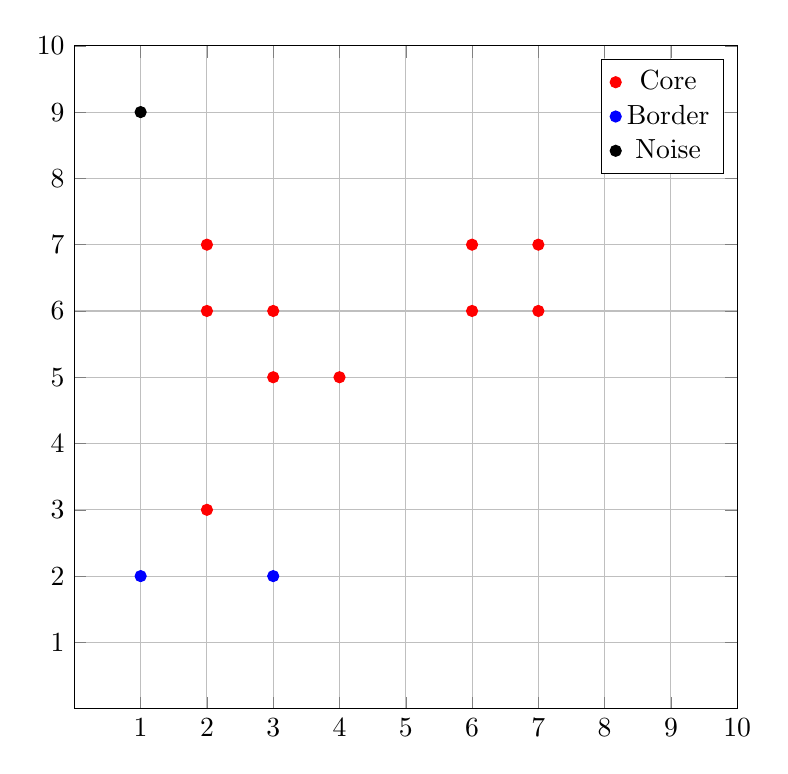
\begin{tikzpicture}
  \begin{axis}[
      xmin=0, xmax=10,
      ymin=0, ymax=10,
      width=10cm,
      height=10cm,
      grid=both,
      xtick={1,2,3,4,5,6,7,8,9,10},
      ytick={1,2,3,4,5,6,7,8,9,10}
      ]
      \addplot[
          scatter,only marks,scatter src=explicit symbolic,
          scatter/classes={
              a={red},
              b={blue},
              c={black}
          }
      ]
      table[meta=label] {
      x   y   label
      1   2     b
      1   9     c
      2   3     a
      2   6     a
      2   7     a
      3   2     b
      3   5     a
      3   6     a
      4   5     a
      6   6     a
      6   7     a
      7   6     a
      7   7     a
      };
      \legend{Core,Border,Noise}
  \end{axis}
\end{tikzpicture}

\subsection{b}
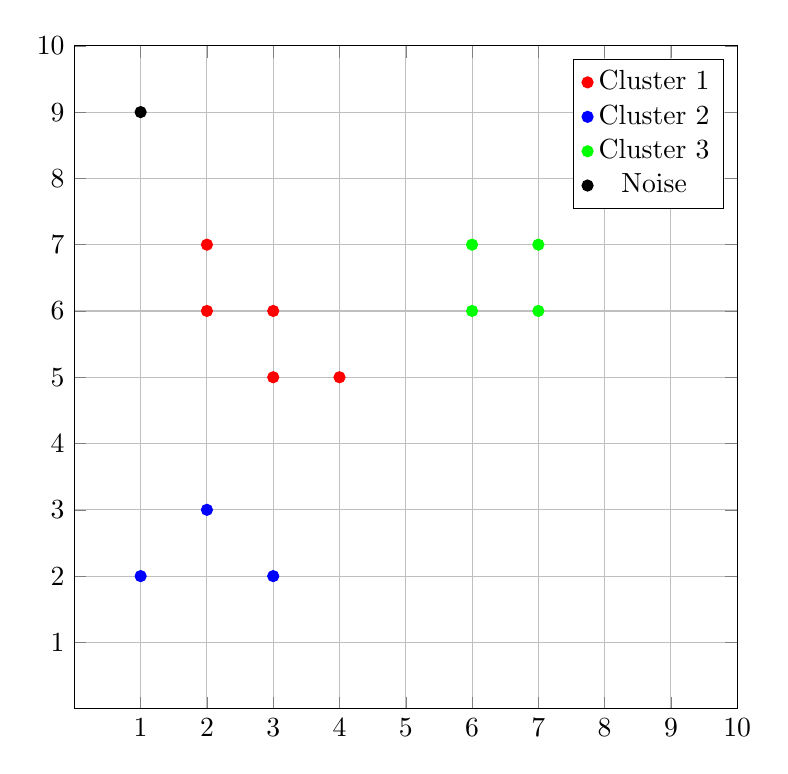
\begin{tikzpicture}
  \begin{axis}[
      xmin=0, xmax=10,
      ymin=0, ymax=10,
      width=10cm,
      height=10cm,
      grid=both,
      xtick={1,2,3,4,5,6,7,8,9,10},
      ytick={1,2,3,4,5,6,7,8,9,10}
      ]
      \addplot[
          scatter,only marks,scatter src=explicit symbolic,
          scatter/classes={
              a={red},
              b={blue},
              c={green},
              d={black}
          }
      ]
      table[meta=label] {
      x   y   label
      1   2     b
      1   9     d
      2   3     b
      2   6     a
      2   7     a
      3   2     b
      3   5     a
      3   6     a
      4   5     a
      6   6     c
      6   7     c
      7   6     c
      7   7     c
      };
      \legend{Cluster 1,Cluster 2,Cluster 3,Noise}
  \end{axis}
\end{tikzpicture}

\subsection{c}
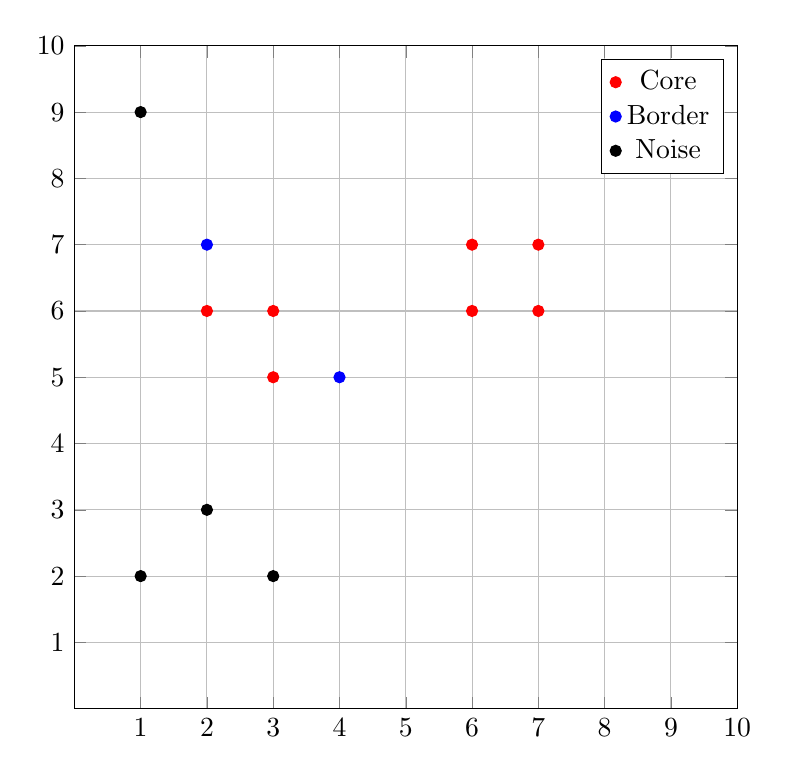
\begin{tikzpicture}
  \begin{axis}[
      xmin=0, xmax=10,
      ymin=0, ymax=10,
      width=10cm,
      height=10cm,
      grid=both,
      xtick={1,2,3,4,5,6,7,8,9,10},
      ytick={1,2,3,4,5,6,7,8,9,10}
      ]
      \addplot[
          scatter,only marks,scatter src=explicit symbolic,
          scatter/classes={
              a={red},
              b={blue},
              c={black}
          }
      ]
      table[meta=label] {
      x   y   label
      1   2     c
      1   9     c
      2   3     c
      2   6     a
      2   7     b
      3   2     c
      3   5     a
      3   6     a
      4   5     b
      6   6     a
      6   7     a
      7   6     a
      7   7     a
      };
      \legend{Core,Border,Noise}
  \end{axis}
\end{tikzpicture}
Compared to part (a), the 3 points in the bottom left have all become outliers
since the point (2,3) is no longer within distance of the other 2 points (Since
the distance between diagonal points is $\sqrt{2}$ away from each other and that
is greater than $\epsilon=1$). Also, the points (2,7) and (4,5) are now border
points because of the same issue with diagonal points. For all of these points,
the number of points within distance $\epsilon=1$ has changed and is now less
than $minpts=3$, causing them to become an outlier if they are within
distance of a core point and they become a border point otherwise.

\subsection{d}
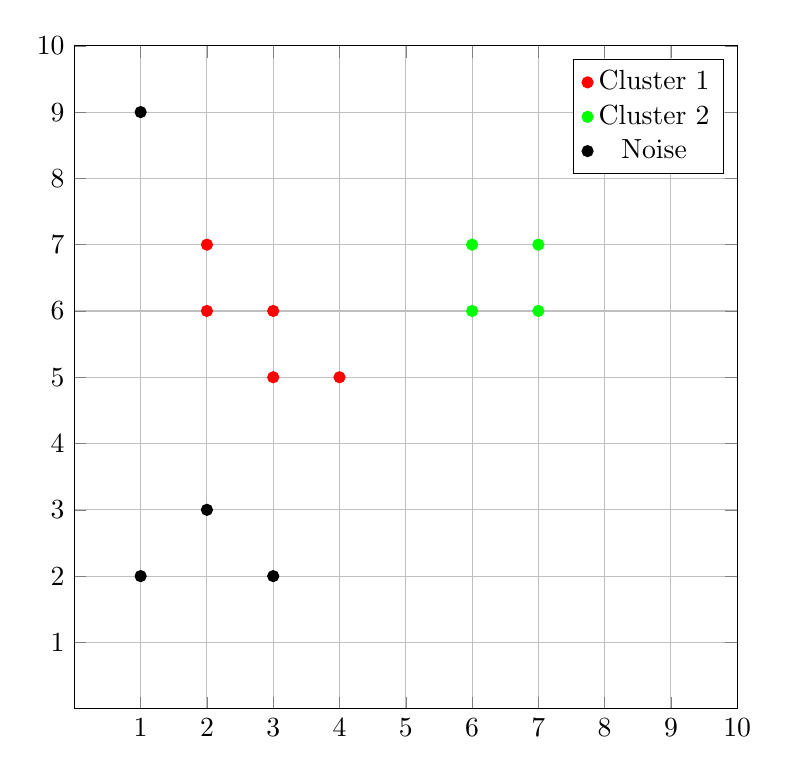
\begin{tikzpicture}
  \begin{axis}[
      xmin=0, xmax=10,
      ymin=0, ymax=10,
      width=10cm,
      height=10cm,
      grid=both,
      xtick={1,2,3,4,5,6,7,8,9,10},
      ytick={1,2,3,4,5,6,7,8,9,10}
      ]
      \addplot[
          scatter,only marks,scatter src=explicit symbolic,
          scatter/classes={
              a={red},
              b={green},
              c={black}
          }
      ]
      table[meta=label] {
      x   y   label
      1   2     c
      1   9     c
      2   3     c
      2   6     a
      2   7     a
      3   2     c
      3   5     a
      3   6     a
      4   5     a
      6   6     b
      6   7     b
      7   6     b
      7   7     b
      };
      \legend{Cluster 1,Cluster 2,Noise}
  \end{axis}
\end{tikzpicture}
Compared to part (b), the bottom left points are no longer a single cluster
since these points became outliers and are not connected.

\end{document}
